\documentclass[12pt,]{article}
\usepackage{lmodern}
\usepackage{amssymb,amsmath}
\usepackage{ifxetex,ifluatex}
\usepackage{fixltx2e} % provides \textsubscript
\ifnum 0\ifxetex 1\fi\ifluatex 1\fi=0 % if pdftex
  \usepackage[T1]{fontenc}
  \usepackage[utf8]{inputenc}
\else % if luatex or xelatex
  \ifxetex
    \usepackage{mathspec}
  \else
    \usepackage{fontspec}
  \fi
  \defaultfontfeatures{Ligatures=TeX,Scale=MatchLowercase}
\fi
% use upquote if available, for straight quotes in verbatim environments
\IfFileExists{upquote.sty}{\usepackage{upquote}}{}
% use microtype if available
\IfFileExists{microtype.sty}{%
\usepackage[]{microtype}
\UseMicrotypeSet[protrusion]{basicmath} % disable protrusion for tt fonts
}{}
\PassOptionsToPackage{hyphens}{url} % url is loaded by hyperref
\usepackage[unicode=true]{hyperref}
\hypersetup{
            pdfborder={0 0 0},
            breaklinks=true}
\urlstyle{same}  % don't use monospace font for urls
\usepackage[margin=1in]{geometry}
\usepackage{graphicx,grffile}
\makeatletter
\def\maxwidth{\ifdim\Gin@nat@width>\linewidth\linewidth\else\Gin@nat@width\fi}
\def\maxheight{\ifdim\Gin@nat@height>\textheight\textheight\else\Gin@nat@height\fi}
\makeatother
% Scale images if necessary, so that they will not overflow the page
% margins by default, and it is still possible to overwrite the defaults
% using explicit options in \includegraphics[width, height, ...]{}
\setkeys{Gin}{width=\maxwidth,height=\maxheight,keepaspectratio}
\IfFileExists{parskip.sty}{%
\usepackage{parskip}
}{% else
\setlength{\parindent}{0pt}
\setlength{\parskip}{6pt plus 2pt minus 1pt}
}
\setlength{\emergencystretch}{3em}  % prevent overfull lines
\providecommand{\tightlist}{%
  \setlength{\itemsep}{0pt}\setlength{\parskip}{0pt}}
\setcounter{secnumdepth}{0}
% Redefines (sub)paragraphs to behave more like sections
\ifx\paragraph\undefined\else
\let\oldparagraph\paragraph
\renewcommand{\paragraph}[1]{\oldparagraph{#1}\mbox{}}
\fi
\ifx\subparagraph\undefined\else
\let\oldsubparagraph\subparagraph
\renewcommand{\subparagraph}[1]{\oldsubparagraph{#1}\mbox{}}
\fi

% set default figure placement to htbp
\makeatletter
\def\fps@figure{htbp}
\makeatother

\usepackage{setspace}\doublespacing
\usepackage{float}
\usepackage{caption}
\usepackage{booktabs}
\usepackage{longtable}
\usepackage{array}
\usepackage{multirow}
\usepackage{wrapfig}
\usepackage{float}
\usepackage{colortbl}
\usepackage{pdflscape}
\usepackage{tabu}
\usepackage{threeparttable}
\usepackage{threeparttablex}
\usepackage[normalem]{ulem}
\usepackage{makecell}
\usepackage{xcolor}

\author{}
\date{\vspace{-2.5em}}

\begin{document}

\captionsetup[figure]{labelformat=empty}
\captionsetup[table]{labelformat=empty} \renewcommand{\figurename}{}

\section{Supporting information:}\label{supporting-information}

\section{Recipient and donor characteristics govern the hierarchical
structure of heterospecific pollen competition
networks}\label{recipient-and-donor-characteristics-govern-the-hierarchical-structure-of-heterospecific-pollen-competition-networks}

\textbf{Authors:} Jose B. Lanuza, Ignasi Bartomeus, Tia-Lynn Ashman,
Romina Rader

The following Supporting Information is available for this article:

\textbf{Table S1.} Species names, common names, varieties and sources of
the different seeds.

\textbf{Table S2.} Numerical values of all the traits measured for each
species.

\textbf{Table S3.} Seed set in percentage for hand cross-pollination,
hand self-pollination, natural selfing and apomixis for all species.

\textbf{Table S4.} Species x species matrix with the significance of
effect ``yes'' or ``no'' of the different donors on the seed set of the
different recipient species.

\textbf{Table S5.} Estimates, standard error, t-value and P-value of the
effect of the different 9 donors on each recipient species.

\textbf{Table S6.} Number of seeds produced with 100\% foreign pollen
treatments for the different recipient species.

\textbf{Table S7.} Phylogenetic signal and significance for all the
different traits

\textbf{Table S8.} Procrustes analysis results.

\textbf{Figure S1}. Total amount of pollen deposited per stigma.

\textbf{Figure S2}. Pollen ratios for the different recipient species.

\textbf{Figure S3}. Pollen ratios for the different recipient species by
family.

\textbf{Figure S4}. Statistical comparison of the pollen ratios by
family.

\textbf{Figure S5}. Unipartite bidirectional network with asymmetrical
effect.

\textbf{Figure S6}. Correlation matrix for all the different traits.

\textbf{Figure S7}. Species reproductive biology.

\textbf{Figure S8}. Grouped effect sizes by family for each recipient
species.

\newpage

\begingroup\fontsize{10}{12}\selectfont

\begin{longtabu} to \linewidth {>{\em}l>{\raggedright}X>{\raggedright}X>{\raggedright}X}
\caption{\label{tab:unnamed-chunk-1}\textbf{Table S1.} Species names, common names, varieties and sources of the different seeds.}\\
\toprule
\textbf{Species} & \textbf{Common names} & \textbf{Varieties} & \textbf{Source}\\
\midrule
\endfirsthead
\caption[]{\textbf{Table S1.} Species names, common names, varieties and sources of the different seeds. \textit{(continued)}}\\
\toprule
Species & Common names & Varieties & Source\\
\midrule
\endhead

\endfoot
\bottomrule
\endlastfoot
\rowcolor{gray!6}  Brassica oleracea & Wild cabbage & Capitata & https://www.mrfothergills.com.au/\\
\addlinespace
Brassica rapa & Pak choi & Chinensis & https://www.mrfothergills.com.au/\\
\addlinespace
\rowcolor{gray!6}  Eruca sativa & Rocket &  & https://www.mrfothergills.com.au/\\
\addlinespace
Sinapis alba & White mustard &  & https://www.mrfothergills.com.au/\\
\addlinespace
\rowcolor{gray!6}  Ipomoea aquatica & Water spinach &  & https://www.theseedcollection.com.au/\\
\addlinespace
Ipomoea purpurea & Morning glory &  & http://www.shaman-australis.com.au\\
\addlinespace
\rowcolor{gray!6}  Capsicum annuum & Capsicum & California Wonder & https://www.edenseeds.com.au\\
\addlinespace
Petunia integrifolia & Petunia &  & https://www.dianeseeds.com/\\
\addlinespace
\rowcolor{gray!6}  Solanum lycopersicum & Tomato & Tommy Toe & https://www.mrfothergills.com.au/\\
\addlinespace
Solanum melongena & Eggplant & Little Fingers & https://www.4seasonsseeds.com.au/\\*
\end{longtabu}

\endgroup{}

\begin{landscape}


\begin{table}

\caption{\label{tab:unnamed-chunk-2}\textbf{Table S2.} Trait measurements ($\bar{X}$ ± SD) for the 13 different traits measured for each plant species. Detailed information of how pollen:ovule ratio, selfing rate and SI index were calculated is available in the plant functional traits section from the methods. }
\centering
\resizebox{\linewidth}{!}{
\fontsize{6}{8}\selectfont
\begin{tabu} to \linewidth {>{\em}l>{\raggedleft}X>{\raggedleft}X>{\raggedleft}X>{\raggedleft}X>{\raggedleft}X>{\raggedleft}X>{\raggedleft}X>{\raggedleft}X>{\raggedleft}X>{\raggedleft}X>{\raggedleft}X>{\raggedleft}X>{\raggedleft}X}
\toprule
\textbf{Species} & \textbf{Pollen size $\mu$m} & \textbf{Pollen grains per anther} & \textbf{Ovule number} & \textbf{Pollen:ovule ratio} & \textbf{Stigma area $\mu$m$^{2}$} & \textbf{Stigma length (mm)} & \textbf{Stigma width (mm)} & \textbf{Style length (mm)} & \textbf{Style width (mm)} & \textbf{Ovary length (mm)} & \textbf{Ovary width (mm)} & \textbf{Selfing rate} & \textbf{SI index}\\
\midrule
\rowcolor{gray!6}  Brassica oleracea & 27.72 & 42033 & 29 & 8696.48 & 0.62 & 0.53 & 0.88 & 2.32 & 0.65 & 5.93 & 1.11 & 0.0 & 0.00\\
\addlinespace
Brassica rapa & 25.35 & 7133 & 26 & 1646.08 & 0.36 & 0.37 & 0.73 & 1.08 & 0.52 & 3.53 & 0.88 & 0.0 & 0.00\\
\addlinespace
\rowcolor{gray!6}  Capsicum annuum & 32.46 & 30761 & 241 & 765.83 & 1.06 & 0.72 & 1.18 & 3.24 & 1.06 & 3.15 & 5.80 & 0.8 & 0.64\\
\addlinespace
Eruca versicaria & 24.95 & 22151 & 24 & 5537.75 & 0.35 & 0.73 & 0.67 & 6.60 & 0.73 & 4.42 & 0.94 & 0.1 & 0.02\\
\addlinespace
\rowcolor{gray!6}  Ipomoea aquatica & 70.10 & 858 & 4 & 1072.50 & 3.26 & 1.43 & 2.25 & 19.44 & 0.45 & 2.38 & 1.42 & 0.6 & 0.75\\
\addlinespace
Ipomoea purpurea & 97.59 & 654 & 6 & 545.00 & 2.27 & 1.24 & 1.88 & 28.23 & 0.58 & 1.06 & 1.57 & 1.0 & 2.74\\
\addlinespace
\rowcolor{gray!6}  Petunia integrifolia & 24.74 & 34657 & 220 & 787.66 & 1.17 & 0.80 & 1.32 & 14.65 & 0.45 & 3.13 & 1.77 & 0.9 & 0.26\\
\addlinespace
Sinapis alba & 33.59 & 3507 & 6 & 3507.00 & 0.55 & 0.63 & 0.91 & 3.62 & 0.77 & 1.98 & 1.07 & 0.7 & 1.12\\
\addlinespace
\rowcolor{gray!6}  Solanum lycopersicum & 22.00 & 28915 & 92 & 1885.76 & 0.09 & 0.19 & 0.35 & 6.47 & 0.31 & 1.16 & 1.13 & 0.7 & 0.48\\
\addlinespace
Solanum melongena & 25.18 & 166989 & 1010 & 992.01 & 1.14 & 0.96 & 1.33 & 11.33 & 0.94 & 4.02 & 3.55 & 1.0 & 1.45\\
\bottomrule
\end{tabu}}
\end{table}

\end{landscape}

\begin{table}

\caption{\label{tab:unnamed-chunk-3}\textbf{Table S3.} Results of the test of hand cross-pollination, hand self-pollination, spontaneous selfing and apomixis for all species. The values provided are the seed:ovule ratios in percentage.}
\centering
\resizebox{\linewidth}{!}{
\fontsize{10}{12}\selectfont
\begin{tabu} to \linewidth {>{\em}l>{\raggedleft}X>{\raggedleft}X>{\raggedleft}X>{\raggedleft}X}
\toprule
\textbf{Species} & \textbf{Hand cross-pollination} & \textbf{Hand self-pollination} & \textbf{Spontaneous selfing} & \textbf{Apomixis}\\
\midrule
\rowcolor{gray!6}  Brassica oleracea & 32.07 & 0.00 & 0.00 & 0\\
\addlinespace
Brassica rapa & 44.97 & 0.00 & 0.00 & 0\\
\addlinespace
\rowcolor{gray!6}  Capsicum annuum & 80.00 & 56.47 & 19.34 & 0\\
\addlinespace
Eruca sativa & 23.75 & 0.42 & 0.00 & 0\\
\addlinespace
\rowcolor{gray!6}  Ipomoea aquatica & 40.00 & 30.00 & 20.00 & 0\\
\addlinespace
Ipomoea purpurea & 31.67 & 86.67 & 31.67 & 0\\
\addlinespace
\rowcolor{gray!6}  Petunia integrifolia & 80.16 & 24.77 & 0.00 & 0\\
\addlinespace
Sinapis alba & 41.67 & 48.33 & 5.00 & 15\\
\addlinespace
\rowcolor{gray!6}  Solanum lycopersium & 85.65 & 41.20 & 68.48 & 0\\
\addlinespace
Solanum melongena & 60.48 & 74.87 & 21.56 & 0\\
\bottomrule
\end{tabu}}
\end{table}

\newpage

\begin{landscape}


\begin{table}

\caption{\label{tab:unnamed-chunk-4}\textbf{Table S4.} Species x species matrix with the significance of effect “yes” or “no” of the different donors on seed set from the linear models. The category of “yes” represents a significant effect of the pollen donor (columns) on the recipient species (rows) and the category of “no” represents a lack of significant seed set reduction in comparison with the control. Significance was tested for all species by comparing the different 50-50 CP-HP pollen treatments with the control treatment of hand cross-pollination with conspecific pollen.}
\centering
\resizebox{\linewidth}{!}{
\fontsize{6}{8}\selectfont
\begin{tabu} to \linewidth {>{\em}l>{\raggedright}X>{\raggedright}X>{\raggedright}X>{\raggedright}X>{\raggedright}X>{\raggedright}X>{\raggedright}X>{\raggedright}X>{\raggedright\arraybackslash}p{1.5cm}>{\raggedright}X>{\raggedright}X}
\toprule
\em{} & \em{Brassica oleracea} & \em{Brassica rapa} & \em{Eruca sativa} & \em{Sinapis alba} & \em{Ipomoea aquatica} & \em{Ipomoea purpurea} & \em{Capsicum annuum} & \em{Petunia integrifolia} & \em{Solanum lycopersicum} & \em{Solanum melongena} & \em{$\%$ of significant effect}\\
\midrule
\rowcolor{gray!6}  B. oleracea &  & Yes & Yes & Yes & Yes & Yes & Yes & Yes & Yes & Yes & 100\\
\addlinespace
B. rapa & No &  & Yes & Yes & Yes & Yes & Yes & Yes & Yes & Yes & 88.9\\
\addlinespace
\rowcolor{gray!6}  E. sativa & Yes & No &  & No & Yes & No & No & No & No & No & 22.2\\
\addlinespace
S. alba & No & Yes & No &  & Yes & Yes & Yes & No & No & No & 44.4\\
\addlinespace
\rowcolor{gray!6}  I. aquatica & Yes & Yes & Yes & Yes &  & Yes & Yes & Yes & Yes & Yes & 100\\
\addlinespace
I. purpurea & No & No & Yes & No & No &  & Yes & No & Yes & No & 33.3\\
\addlinespace
\rowcolor{gray!6}  C. annuum & Yes & Yes & No & Yes & No & Yes &  & Yes & Yes1 & Yes & 77.8\\
\addlinespace
P. integrifolia & Yes & No & No & Yes & Yes & Yes & No &  & Yes & Yes & 67.7\\
\addlinespace
\rowcolor{gray!6}  S. lycopersicum & No & Yes & Yes & Yes & Yes & Yes & Yes & Yes &  & Yes & 88.9\\
\addlinespace
S. melongena & No & Yes & Yes & No & Yes & Yes & Yes & No & No &  & 55.6\\
\addlinespace
\rowcolor{gray!6}   &  &  &  &  &  &  &  &  &  &  & $\bar{X}=67.8$\\
\bottomrule
\end{tabu}}
\end{table}

\end{landscape}

\clearpage

\begingroup\fontsize{7}{9}\selectfont

\begin{longtable}[t]{>{\em}lrrrr}
\caption{\label{tab:unnamed-chunk-5}\textbf{Table S5.} Results of the linear models conducted to test heterospecific pollen effect with the 50-50 CP-HP pollen treatments. We conducted 10 different linear models (M1, M2, M3, M4, M5, M6, M7 M8, M9 and M10) where the effect of the different 9 pollen donors was compared with the control treatment of hand cross pollination with conspecific pollen for each recipient species (intercept). The first species on the row names are the pollen recipient species and the second species the pollen donor species. Each treatment is compared with the control or reference treatment that is indicated with the recipient species names and the intercept term between parentheses}\\
\toprule
\textbf{ } & \textbf{Estimates} & \textbf{Standard error} & \textbf{t-value} & \textbf{{\textit{P}}-value}\\
\midrule
\rowcolor{gray!6}  M1 Petunia integrifolia - (Intercept) & 4.63 & 0.49 & 9.36 & 0.00\\
\addlinespace
M1 Petunia integrifolia - Brassica oleracea & -1.84 & 0.81 & -2.27 & 0.03\\
\addlinespace
\rowcolor{gray!6}  M1 Petunia integrifolia - Brassica rapa & -0.97 & 0.81 & -1.19 & 0.24\\
\addlinespace
M1 Petunia integrifolia - Capsicum annuum & 0.78 & 0.81 & 0.96 & 0.34\\
\addlinespace
\rowcolor{gray!6}  M1 Petunia integrifolia - Eruca vesicaria & -0.91 & 0.81 & -1.12 & 0.26\\
\addlinespace
M1 Petunia integrifolia - Ipomoea aquatica & -3.18 & 0.81 & -3.92 & 0.00\\
\addlinespace
\rowcolor{gray!6}  M1 Petunia integrifolia - Ipomoea purpurea & -4.21 & 0.81 & -5.19 & 0.00\\
\addlinespace
M1 Petunia integrifolia - Sinapis alba & -2.99 & 0.81 & -3.69 & 0.00\\
\addlinespace
\rowcolor{gray!6}  M1 Petunia integrifolia - Solanum lycopersicum & -2.40 & 0.81 & -2.96 & 0.00\\
\addlinespace
M1 Petunia integrifolia - Solanum melongena & -2.66 & 0.81 & -3.27 & 0.00\\
\addlinespace
\rowcolor{gray!6}  M2 Solanum lycopersicum - (Intercept) & 4.39 & 0.24 & 18.54 & 0.00\\
\addlinespace
M2 Solanum lycopersicum - Brassica oleracea & -0.47 & 0.41 & -1.14 & 0.26\\
\addlinespace
\rowcolor{gray!6}  M2 Solanum lycopersicum - Brassica rapa & -2.74 & 0.41 & -6.67 & 0.00\\
\addlinespace
M2 Solanum lycopersicum - Capsicum annuum & -4.39 & 0.41 & -10.71 & 0.00\\
\addlinespace
\rowcolor{gray!6}  M2 Solanum lycopersicum - Eruca vesicaria & -2.97 & 0.41 & -7.25 & 0.00\\
\addlinespace
M2 Solanum lycopersicum - Ipomoea aquatica & -4.13 & 0.41 & -10.06 & 0.00\\
\addlinespace
\rowcolor{gray!6}  M2 Solanum lycopersicum - Ipomoea purpurea & -3.80 & 0.41 & -9.27 & 0.00\\
\addlinespace
M2 Solanum lycopersicum - Petunia integrifolia & -1.82 & 0.41 & -4.44 & 0.00\\
\addlinespace
\rowcolor{gray!6}  M2 Solanum lycopersicum - Sinapis alba & -3.72 & 0.41 & -9.08 & 0.00\\
\addlinespace
M2 Solanum lycopersicum - Solanum melongena & -1.84 & 0.41 & -4.49 & 0.00\\
\addlinespace
\rowcolor{gray!6}  M3 Solanum melongena - (Intercept) & 6.34 & 0.70 & 9.09 & 0.00\\
\addlinespace
M3 Solanum melongena - Brassica oleracea & -0.67 & 0.99 & -0.68 & 0.50\\
\addlinespace
\rowcolor{gray!6}  M3 Solanum melongena - Brassica rapa & -4.33 & 0.99 & -4.39 & 0.00\\
\addlinespace
M3 Solanum melongena - Capsicum annuum & -2.33 & 0.99 & -2.36 & 0.02\\
\addlinespace
\rowcolor{gray!6}  M3 Solanum melongena - Eruca vesicaria & -3.12 & 0.99 & -3.16 & 0.00\\
\addlinespace
M3 Solanum melongena - Ipomoea aquatica & -6.34 & 0.99 & -6.43 & 0.00\\
\addlinespace
\rowcolor{gray!6}  M3 Solanum melongena - Ipomoea purpurea & -2.71 & 0.99 & -2.74 & 0.01\\
\addlinespace
M3 Solanum melongena - Petunia integrifolia & -1.43 & 0.99 & -1.45 & 0.15\\
\addlinespace
\rowcolor{gray!6}  M3 Solanum melongena - Sinapis alba & -1.11 & 0.99 & -1.12 & 0.26\\
\addlinespace
M3 Solanum melongena - Solanum lycopersicum & -0.84 & 0.99 & -0.86 & 0.39\\
\addlinespace
\rowcolor{gray!6}  M4 Capsicum annuum - (Intercept) & 4.59 & 0.52 & 8.78 & 0.00\\
\addlinespace
M4 Capsicum annuum - Brassica oleracea & -1.80 & 0.74 & -2.43 & 0.02\\
\addlinespace
\rowcolor{gray!6}  M4 Capsicum annuum - Brassica rapa & -2.51 & 0.74 & -3.39 & 0.00\\
\addlinespace
M4 Capsicum annuum - Eruca vesicaria & -0.63 & 0.74 & -0.85 & 0.40\\
\addlinespace
\rowcolor{gray!6}  M4 Capsicum annuum - Ipomoea aquatica & -1.36 & 0.74 & -1.84 & 0.07\\
\addlinespace
M4 Capsicum annuum - Ipomoea purpurea & -4.00 & 0.74 & -5.41 & 0.00\\
\addlinespace
\rowcolor{gray!6}  M4 Capsicum annuum - Petunia integrifolia & -4.59 & 0.74 & -6.21 & 0.00\\
\addlinespace
M4 Capsicum annuum - Sinapis alba & -3.63 & 0.74 & -4.92 & 0.00\\
\addlinespace
\rowcolor{gray!6}  M4 Capsicum annuum - Solanum lycopersicum & -1.52 & 0.74 & -2.06 & 0.04\\
\addlinespace
M4 Capsicum annuum - Solanum melongena & -3.29 & 0.74 & -4.46 & 0.00\\
\addlinespace
\rowcolor{gray!6}  M5 Brassica oleracea - (Intercept) & 1.99 & 0.22 & 8.98 & 0.00\\
\addlinespace
M5 Brassica oleracea - Brassica rapa & -1.37 & 0.31 & -4.35 & 0.00\\
\addlinespace
\rowcolor{gray!6}  M5 Brassica oleracea - Capsicum annuum & -0.87 & 0.31 & -2.76 & 0.01\\
\addlinespace
M5 Brassica oleracea - Eruca vesicaria & -1.92 & 0.31 & -6.13 & 0.00\\
\addlinespace
\rowcolor{gray!6}  M5 Brassica oleracea - Ipomoea aquatica & -1.91 & 0.27 & -7.04 & 0.00\\
\addlinespace
M5 Brassica oleracea - Ipomoea purpurea & -1.99 & 0.31 & -6.35 & 0.00\\
\addlinespace
\rowcolor{gray!6}  M5 Brassica oleracea - Petunia integrifolia & -1.64 & 0.31 & -5.21 & 0.00\\
\addlinespace
M5 Brassica oleracea - Sinapis alba & -1.57 & 0.31 & -4.99 & 0.00\\
\addlinespace
\rowcolor{gray!6}  M5 Brassica oleracea - Solanum lycopersicum & -1.47 & 0.31 & -4.70 & 0.00\\
\addlinespace
M5 Brassica oleracea - Solanum melongena & -1.61 & 0.31 & -5.12 & 0.00\\
\addlinespace
\rowcolor{gray!6}  M6 Brassica rapa - (Intercept) & 2.37 & 0.19 & 12.49 & 0.00\\
\addlinespace
M6 Brassica rapa - Brassica oleracea & -0.54 & 0.29 & -1.89 & 0.06\\
\addlinespace
\rowcolor{gray!6}  M6 Brassica rapa - Capsicum annuum & -1.42 & 0.29 & -4.94 & 0.00\\
\addlinespace
M6 Brassica rapa - Eruca vesicaria & -2.37 & 0.29 & -8.24 & 0.00\\
\addlinespace
\rowcolor{gray!6}  M6 Brassica rapa - Ipomoea aquatica & -1.92 & 0.29 & -6.67 & 0.00\\
\addlinespace
M6 Brassica rapa - Ipomoea purpurea & -2.26 & 0.29 & -7.86 & 0.00\\
\addlinespace
\rowcolor{gray!6}  M6 Brassica rapa - Petunia integrifolia & -2.37 & 0.29 & -8.24 & 0.00\\
\addlinespace
M6 Brassica rapa - Sinapis alba & -2.37 & 0.29 & -8.24 & 0.00\\
\addlinespace
\rowcolor{gray!6}  M6 Brassica rapa - Solanum lycopersicum & -1.88 & 0.29 & -6.55 & 0.00\\
\addlinespace
M6 Brassica rapa - Solanum melongena & -2.37 & 0.29 & -8.24 & 0.00\\
\addlinespace
\rowcolor{gray!6}  M8 Eruca sativa - (Intercept) & 1.34 & 0.35 & 3.80 & 0.00\\
\addlinespace
M8 Eruca sativa - Brassica oleracea & -1.34 & 0.50 & -2.69 & 0.01\\
\addlinespace
\rowcolor{gray!6}  M8 Eruca sativa - Brassica rapa & 0.66 & 0.50 & 1.32 & 0.19\\
\addlinespace
M8 Eruca sativa - Capsicum annuum & -0.27 & 0.50 & -0.55 & 0.58\\
\addlinespace
\rowcolor{gray!6}  M8 Eruca sativa - Ipomoea aquatica & 0.87 & 0.50 & 1.75 & 0.08\\
\addlinespace
M8 Eruca sativa - Ipomoea purpurea & -0.19 & 0.50 & -0.39 & 0.70\\
\addlinespace
\rowcolor{gray!6}  M8 Eruca sativa - Petunia integrifolia & 0.20 & 0.50 & 0.41 & 0.68\\
\addlinespace
M8 Eruca sativa - Sinapis alba & 0.32 & 0.50 & 0.65 & 0.52\\
\addlinespace
\rowcolor{gray!6}  M8 Eruca sativa - Solanum lycopersicum & -0.52 & 0.50 & -1.04 & 0.30\\
\addlinespace
M8 Eruca sativa - Solanum melongena & 0.54 & 0.50 & 1.09 & 0.28\\
\addlinespace
\rowcolor{gray!6}  M9 Ipomoea purpurea - (Intercept) & 0.82 & 0.20 & 4.05 & 0.00\\
\addlinespace
M9 Ipomoea purpurea - Brassica oleracea & 0.37 & 0.29 & 1.31 & 0.19\\
\addlinespace
\rowcolor{gray!6}  M9 Ipomoea purpurea - Brassica rapa & -0.41 & 0.29 & -1.43 & 0.16\\
\addlinespace
M9 Ipomoea purpurea - Capsicum annuum & -0.82 & 0.29 & -2.86 & 0.01\\
\addlinespace
\rowcolor{gray!6}  M9 Ipomoea purpurea - Eruca vesicaria & -0.75 & 0.29 & -2.62 & 0.01\\
\addlinespace
M9 Ipomoea purpurea - Ipomoea aquatica & 0.41 & 0.29 & 1.44 & 0.15\\
\addlinespace
\rowcolor{gray!6}  M9 Ipomoea purpurea - Petunia integrifolia & -0.37 & 0.29 & -1.31 & 0.19\\
\addlinespace
M9 Ipomoea purpurea - Sinapis alba & -0.33 & 0.29 & -1.14 & 0.26\\
\addlinespace
\rowcolor{gray!6}  M9 Ipomoea purpurea - Solanum lycopersicum & -0.82 & 0.29 & -2.86 & 0.01\\
\addlinespace
M9 Ipomoea purpurea - Solanum melongena & -0.24 & 0.29 & -0.82 & 0.41\\
\addlinespace
\rowcolor{gray!6}  M10 Ipomoea aquatica - (Intercept) & 0.80 & 0.09 & 9.36 & 0.00\\
\addlinespace
M10 Ipomoea aquatica - Brassica oleracea & -0.80 & 0.12 & -6.62 & 0.00\\
\addlinespace
\rowcolor{gray!6}  M10 Ipomoea aquatica - Brassica rapa & -0.80 & 0.12 & -6.62 & 0.00\\
\addlinespace
M10 Ipomoea aquatica - Capsicum annuum & -0.80 & 0.12 & -6.62 & 0.00\\
\addlinespace
\rowcolor{gray!6}  M10 Ipomoea aquatica - Eruca vesicaria & -0.80 & 0.12 & -6.62 & 0.00\\
\addlinespace
M10 Ipomoea aquatica - Ipomoea purpurea & -0.80 & 0.12 & -6.62 & 0.00\\
\addlinespace
\rowcolor{gray!6}  M10 Ipomoea aquatica - Petunia integrifolia & -0.59 & 0.12 & -4.89 & 0.00\\
\addlinespace
M10 Ipomoea aquatica - Sinapis alba & -0.80 & 0.12 & -6.62 & 0.00\\
\addlinespace
\rowcolor{gray!6}  M10 Ipomoea aquatica - Solanum lycopersicum & -0.69 & 0.12 & -5.70 & 0.00\\
\addlinespace
M10 Ipomoea aquatica - Solanum melongena & -0.80 & 0.12 & -6.62 & 0.00\\
\bottomrule
\end{longtable}

\endgroup{}

\clearpage

\begin{table}

\caption{\label{tab:unnamed-chunk-6}\textbf{Table S6.} Number of seeds produced with 100\% foreign pollen (N=900). From 900 pollination events we found seed production in just 13 specific cases and 0 seed production in the other 887 pollination events. In this table we show just the treatments that lead to seed production.}
\resizebox{\linewidth}{!}{
\fontsize{10}{12}\selectfont
\begin{tabular}[t]{>{\em}l>{\em}lr}
\toprule
\textbf{Recipient} & \textbf{Donor (100\% foreign pollen)} & \textbf{Seed number}\\
\midrule
\rowcolor{gray!6}  Solnamum lycopersicum & Sinapis alba & 3\\
\addlinespace
Solnamum melongena & Petunia integrifolia & 36\\
\addlinespace
\rowcolor{gray!6}  Capsicum annuum & Eruca sativa & 3\\
\addlinespace
Capsicum annuum & Sinapis alba & 127\\
\addlinespace
\rowcolor{gray!6}  Brassica rapa & Brassica oleracea & 2\\
\addlinespace
Brassica rapa & Brassica oleracea & 13\\
\addlinespace
\rowcolor{gray!6}  Sinapis alba & Brassica oleracea & \vphantom{1} 7\\
\addlinespace
Sinapis alba & Brassica oleracea & 5\\
\addlinespace
\rowcolor{gray!6}  Sinapis alba & Brassica oleracea & \vphantom{1} 7\\
\addlinespace
Sinapis alba & Capsicum annuum & 1\\
\addlinespace
\rowcolor{gray!6}  Sinapis alba & Capsicum annuum & 6\\
\addlinespace
Sinapis alba & Solanum lycopersicum & 1\\
\addlinespace
\rowcolor{gray!6}  Eruca sativa & Petunia integrifolia & 2\\
\bottomrule
\multicolumn{3}{l}{\textsuperscript{} * Note: There are some specific cases that we think that hybridization did not occur and that}\\
\multicolumn{3}{l}{the recipient species were pollen contaminated, like the one of C. annuum with S. alba with 127}\\
\multicolumn{3}{l}{seeds. This seems to be the case for 5 other crosses that had very low seed production when they}\\
\multicolumn{3}{l}{were pollinated with 100\% foreign pollen with species of other family members. This represents}\\
\multicolumn{3}{l}{very few isolated cases (0.67\% of all the 100\% foreign pollen crosses conducted) and we}\\
\multicolumn{3}{l}{think that our results are not compromised by this fact.}\\
\end{tabular}}
\end{table}

\clearpage

\begin{table}

\caption{\label{tab:unnamed-chunk-7}\textbf{Table S7.} Phylogenetic signal and significance for the 13 different reproductive traits measured for all species.}
\centering
\fontsize{10}{12}\selectfont
\begin{tabular}[t]{rrl}
\toprule
\textbf{Lambda} & \textbf{P-value} & \textbf{Traits}\\
\midrule
\rowcolor{gray!6}  0.95 & 0.20 & Selfing rate\\
\addlinespace
1.00 & 0.00 & Pollen size\\
\addlinespace
\rowcolor{gray!6}  0.00 & 1.00 & Pollen anther\\
\addlinespace
0.00 & 1.00 & Ovule number\\
\addlinespace
\rowcolor{gray!6}  0.00 & 1.00 & Pollen-ovule ratio\\
\addlinespace
0.89 & 0.01 & Stigmatic area\\
\addlinespace
\rowcolor{gray!6}  0.70 & 0.05 & Stigma length\\
\addlinespace
0.77 & 0.03 & Stigma width\\
\addlinespace
\rowcolor{gray!6}  0.93 & 0.01 & Style length\\
\addlinespace
0.00 & 1.00 & Style width\\
\addlinespace
\rowcolor{gray!6}  0.47 & 0.30 & Ovary length\\
\addlinespace
0.00 & 1.00 & Ovary width\\
\addlinespace
\rowcolor{gray!6}  0.00 & 0.02 & SI index\\
\bottomrule
\end{tabular}
\end{table}

\clearpage

\begingroup\fontsize{7}{9}\selectfont

\begin{longtable}[t]{rrrll}
\caption{\label{tab:unnamed-chunk-8}\textbf{Table S8.} Procrustes correlation, sum of squares and significance from Procrustes analysis between the matrix of effect sizes (species x species matrix) and the distance matrix of each trait for all families, just Solanaceae family and just Brassicaceae family.}\\
\toprule
\textbf{Correlation (r)} & \textbf{Sum of squares} & \textbf{P-value} & \textbf{Traits} & \textbf{Family}\\
\midrule
\rowcolor{gray!6}  0.34 & 0.88 & 0.70 & Selfing rate & All\\
\addlinespace
0.36 & 0.87 & 0.42 & Pollen size & All\\
\addlinespace
\rowcolor{gray!6}  0.35 & 0.88 & 0.57 & Pollen per anther & All\\
\addlinespace
0.33 & 0.89 & 0.55 & Number of ovules & All\\
\addlinespace
\rowcolor{gray!6}  0.30 & 0.91 & 0.86 & Pollen-ovule ratio & All\\
\addlinespace
0.37 & 0.86 & 0.68 & Stigmatic area & All\\
\addlinespace
\rowcolor{gray!6}  0.62 & 0.62 & 0.10 & Stigma length & All\\
\addlinespace
0.46 & 0.79 & 0.47 & Stigma width & All\\
\addlinespace
\rowcolor{gray!6}  0.43 & 0.82 & 0.45 & Style length & All\\
\addlinespace
0.59 & 0.65 & 0.11 & Style width & All\\
\addlinespace
\rowcolor{gray!6}  0.34 & 0.88 & 0.57 & Ovary length & All\\
\addlinespace
0.35 & 0.88 & 0.93 & Ovary width & All\\
\addlinespace
\rowcolor{gray!6}  0.49 & 0.76 & 0.24 & Self-incompatibility index & All\\
\addlinespace
0.86 & 0.26 & 0.25 & Selfing rate & Solanaceae\\
\addlinespace
\rowcolor{gray!6}  0.76 & 0.42 & 0.33 & Pollen size & Solanaceae\\
\addlinespace
0.42 & 0.82 & 0.79 & Pollen per anther & Solanaceae\\
\addlinespace
\rowcolor{gray!6}  0.52 & 0.73 & 0.83 & Number of ovules & Solanaceae\\
\addlinespace
0.87 & 0.25 & 0.04 & Pollen-ovule ratio & Solanaceae\\
\addlinespace
\rowcolor{gray!6}  0.82 & 0.33 & 0.17 & Stigmatic area & Solanaceae\\
\addlinespace
0.89 & 0.20 & 0.08 & Stigma length & Solanaceae\\
\addlinespace
\rowcolor{gray!6}  0.84 & 0.29 & 0.12 & Stigma width & Solanaceae\\
\addlinespace
0.78 & 0.39 & 0.50 & Style length & Solanaceae\\
\addlinespace
\rowcolor{gray!6}  0.52 & 0.73 & 0.71 & Style width & Solanaceae\\
\addlinespace
0.64 & 0.60 & 0.79 & Ovary length & Solanaceae\\
\addlinespace
\rowcolor{gray!6}  0.87 & 0.23 & 0.17 & Ovary width & Solanaceae\\
\addlinespace
0.50 & 0.75 & 1.00 & Self-incompatibility index & Solanaceae\\
\addlinespace
\rowcolor{gray!6}  0.61 & 0.63 & 0.50 & Selfing rate & Brassicaceae\\
\addlinespace
0.60 & 0.64 & 0.71 & Pollen size & Brassicaceae\\
\addlinespace
\rowcolor{gray!6}  0.40 & 0.84 & 0.96 & Pollen per anther & Brassicaceae\\
\addlinespace
0.62 & 0.61 & 0.42 & Number of ovules & Brassicaceae\\
\addlinespace
\rowcolor{gray!6}  0.49 & 0.76 & 0.96 & Pollen-ovule ratio & Brassicaceae\\
\addlinespace
0.55 & 0.70 & 0.58 & Stigmatic area & Brassicaceae\\
\addlinespace
\rowcolor{gray!6}  0.92 & 0.15 & 0.08 & Stigma length & Brassicaceae\\
\addlinespace
0.63 & 0.60 & 0.38 & Stigma width & Brassicaceae\\
\addlinespace
\rowcolor{gray!6}  0.83 & 0.31 & 0.08 & Style length & Brassicaceae\\
\addlinespace
0.79 & 0.37 & 0.33 & Style width & Brassicaceae\\
\addlinespace
\rowcolor{gray!6}  0.59 & 0.65 & 0.50 & Ovary length & Brassicaceae\\
\addlinespace
0.54 & 0.70 & 1.00 & Ovary width & Brassicaceae\\
\addlinespace
\rowcolor{gray!6}  0.50 & 0.75 & 0.83 & Self-incompatibility index & Brassicaceae\\
\bottomrule
\end{longtable}

\endgroup{}

\clearpage

\begin{figure}
\centering
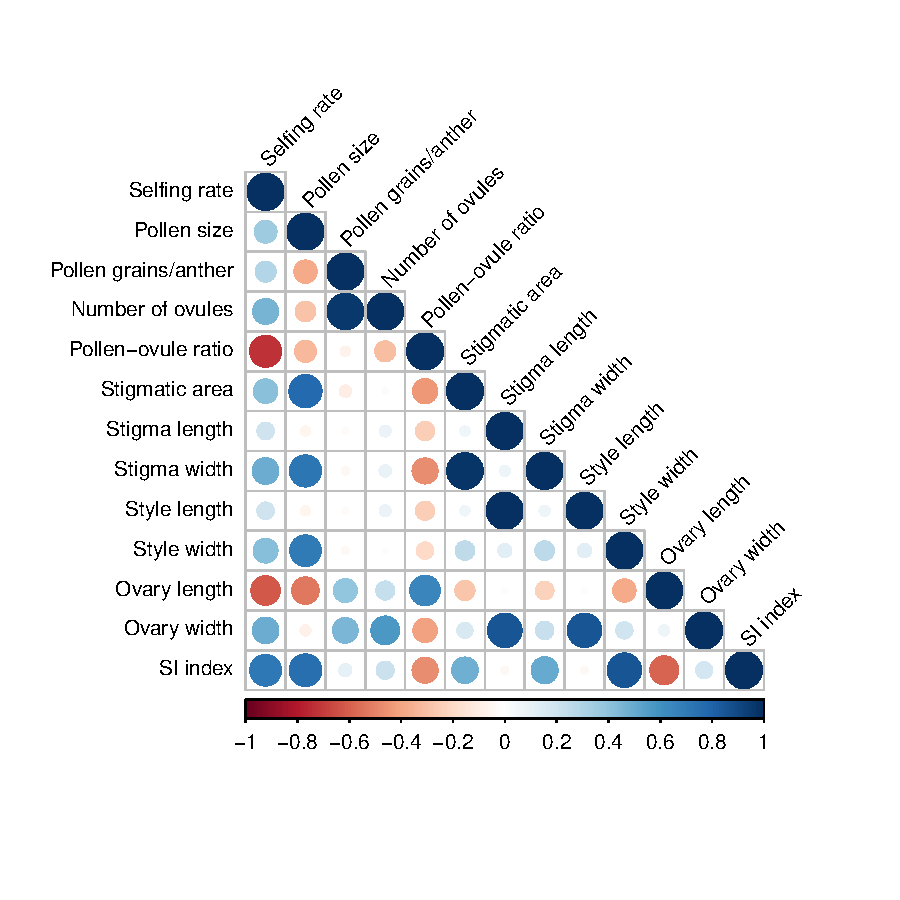
\includegraphics{Supp_Material_files/figure-latex/unnamed-chunk-9-1.pdf}
\caption{\textbf{Fig. S1} Average number of pollen grains per stigma for
20 different treatments (3 replicates per tratment). For each treatment,
we show the average number of conspecific pollen grains (grey) and
heterospecific pollen grains (light blue) per stigma. For each pair of
species on the x-axis, the first species is the recipient species, and
the second, the donor species.}
\end{figure}

\clearpage

\begin{figure}
\centering
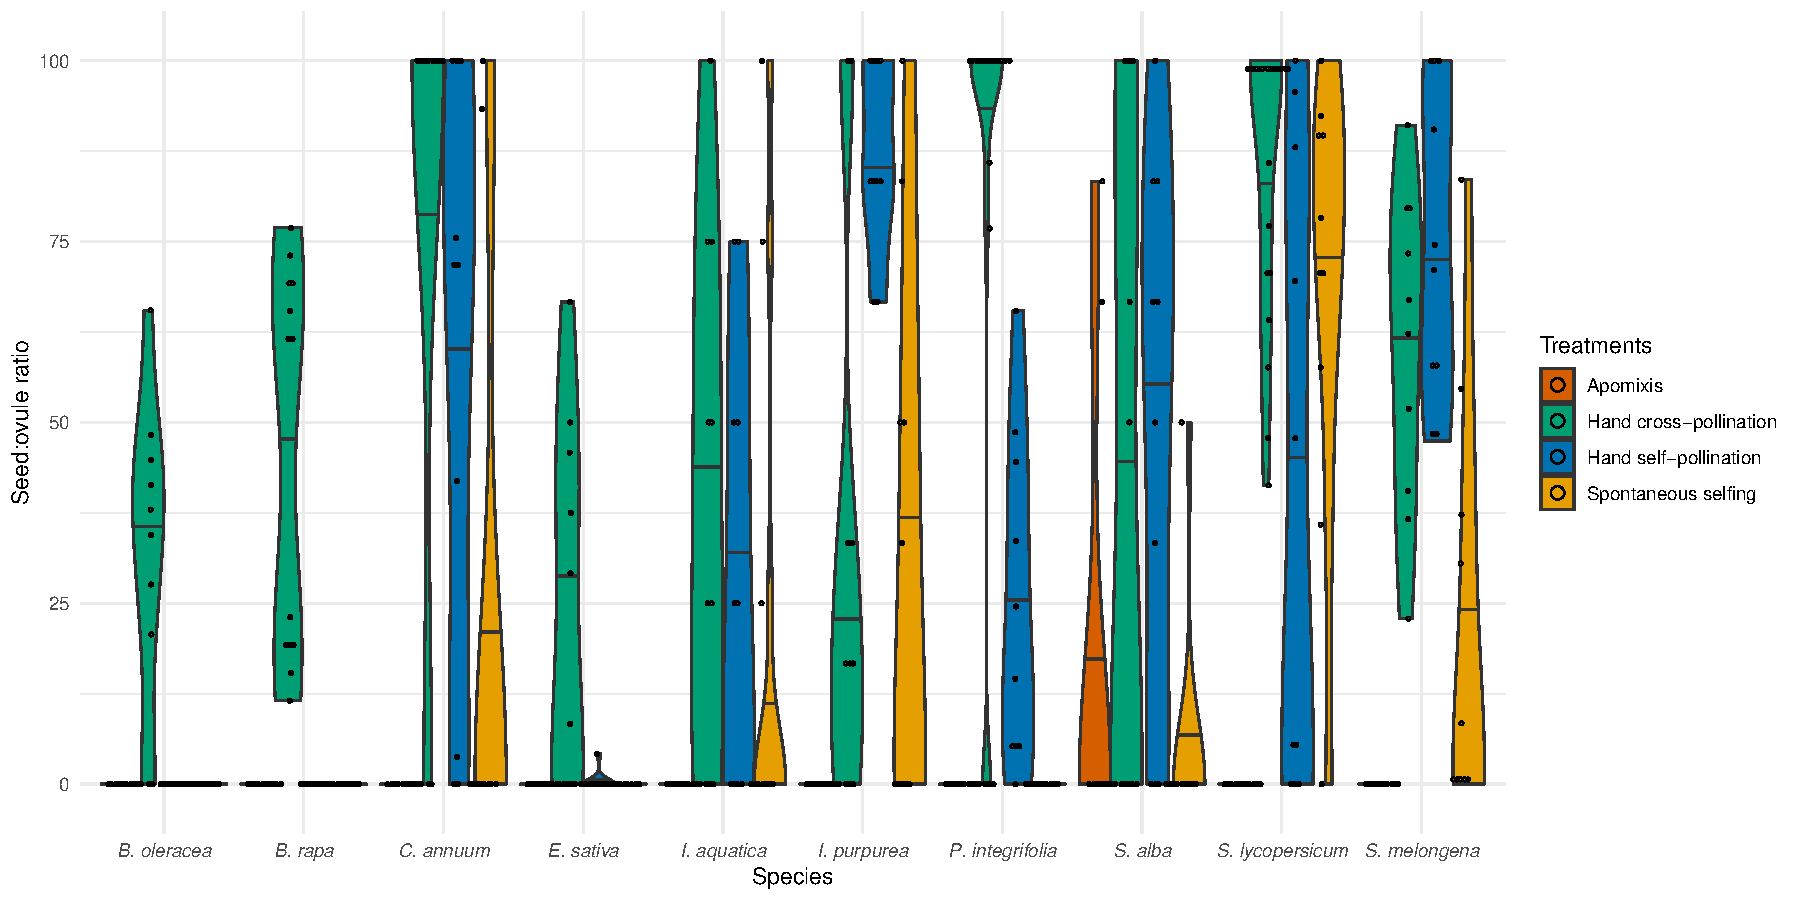
\includegraphics{Supp_Material_files/figure-latex/unnamed-chunk-10-1.pdf}
\caption{\textbf{Fig. S2} Average proportion of conspecific and
heterospecific pollen per stigma grouped by family, A) Brassicaceae, B)
Solanaceae and C) Convolvulaceae. These proportions (\%) are the number
of conspecific pollen grains or heterospecific pollen grains divided by
the total number of pollen grains per stigma for 20 different
treatments. We conducted 3 count replicates per treatment and then we
calculated the average number of pollen grains for these treatments. The
proportion of conspecific and heterospecific pollen are shown in grey
and light blue respectively. For each pair of species on the y-axis, the
first species is the pollen recipient and the second the pollen donor.
The vertical black line represents 50\% pollen of both donor and
recipient.}
\end{figure}

\clearpage

\begin{figure}
\centering
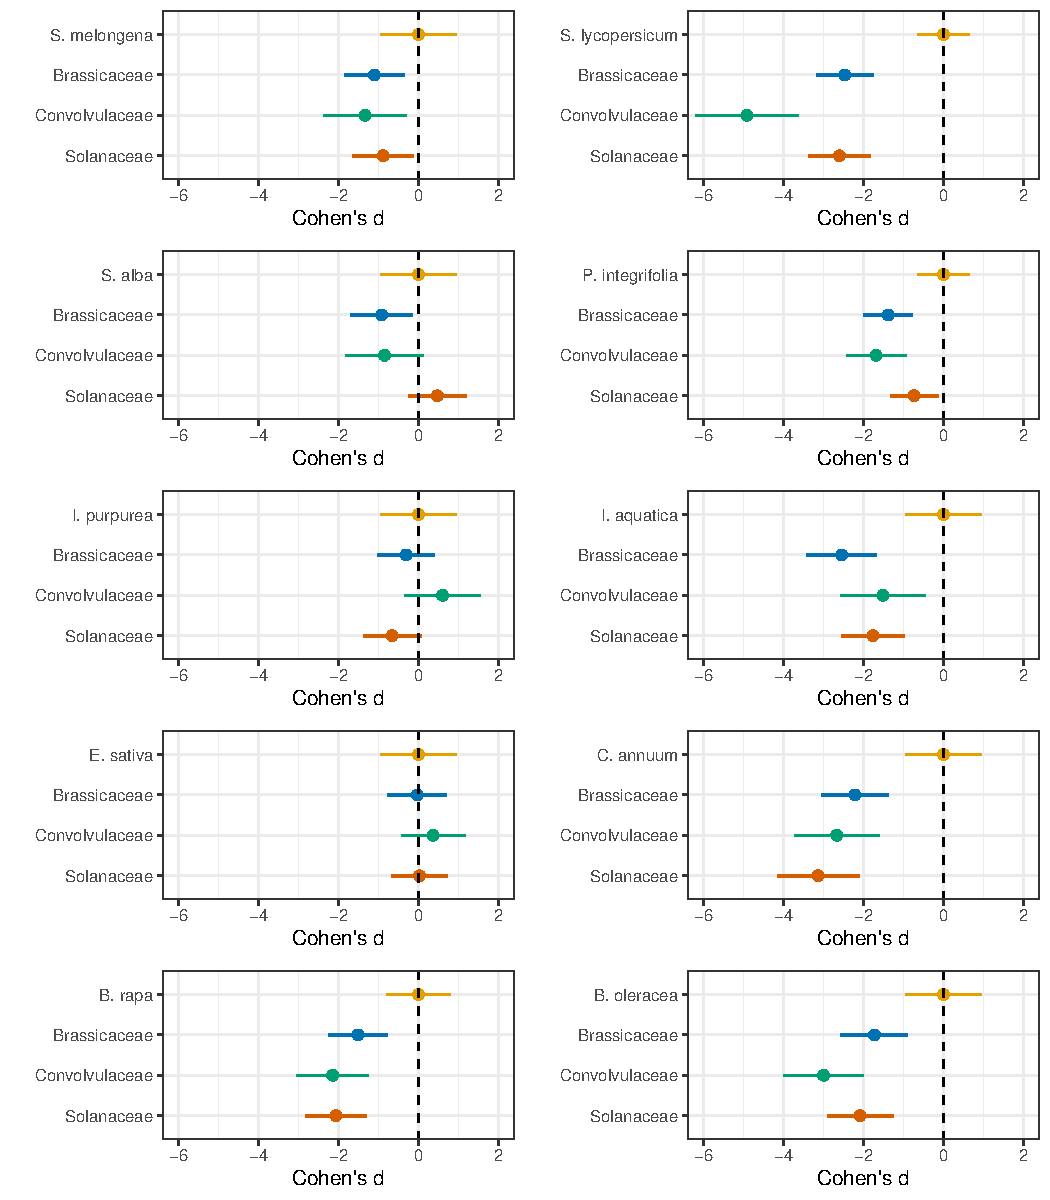
\includegraphics{Supp_Material_files/figure-latex/unnamed-chunk-11-1.pdf}
\caption{\textbf{Fig. S3} Average proportion (\%) of heterospecific and
conspecific pollen per family for the different 20 treatments counted.
We conducted 3 count replicates per treatment and then we calculated the
average number of pollen grains for these different 20 treatments.
Finally, we grouped by family these treatments in order to see general
tendencies across families as pollen donor and as pollen recipient.
Pollen ratios were considered as the number of conspecific or
heterospecific pollen grains divided by the total number of pollen
grains per stigma. On the y-axis, the first family on each pair of plant
families is the recipient one, and the second, the family of the donor.
The vertical bar on intercept 50, represents equal proportions of both
recipient (grey) and donor (light blue) pollen.}
\end{figure}

\clearpage

\begin{figure}
\centering
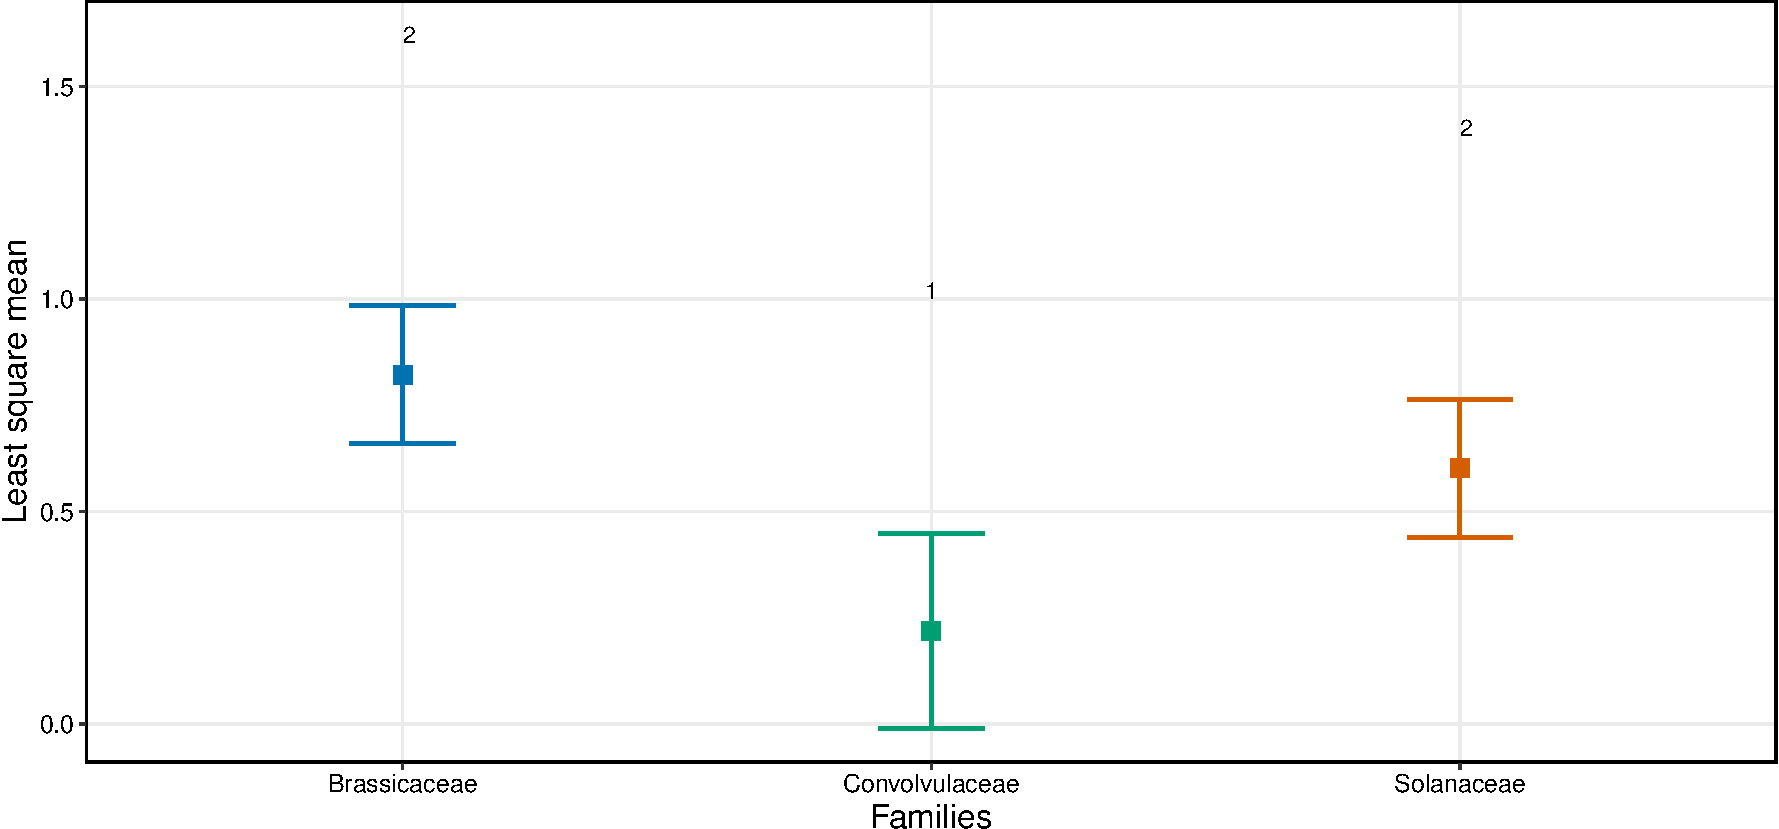
\includegraphics{Supp_Material_files/figure-latex/unnamed-chunk-12-1.pdf}
\caption{\textbf{Fig. S4} Pollen ratios comparisons between the
different pollen recipient families where the boxes represent least
square means, the error bars, confidence intervals 95\%, and sharing
numbers indicate no significant differences between groups (Tukey
adjusted comparisons). These pollen ratios (\%) are the total number of
heterospecific pollen grains divided by the total quantity of pollen
(conspecific pollen + heterospecific pollen), and then compared by
family (N=20). Brassicacea family is coloured in blue, Convolvulaceae in
green and Solanaceae in orange.}
\end{figure}

\newpage

\begin{figure}
\centering
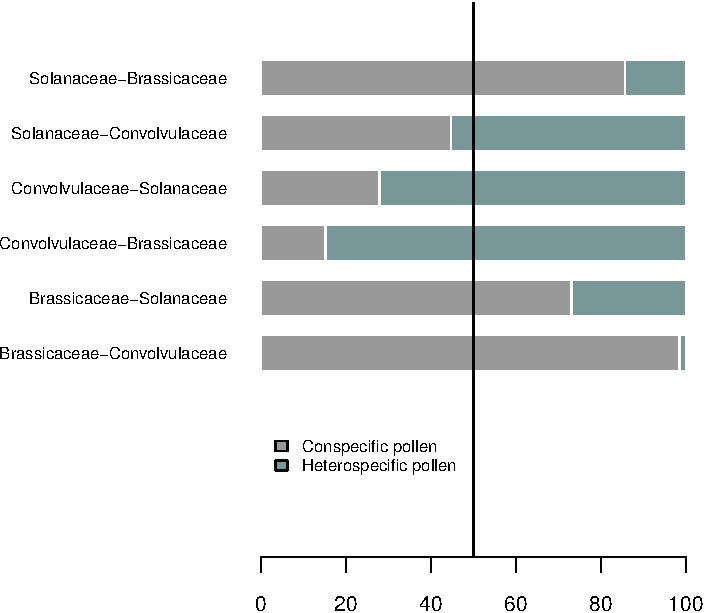
\includegraphics{Supp_Material_files/figure-latex/unnamed-chunk-13-1.pdf}
\caption{\textbf{Fig. S5} Unipartite bidirectional network with
asymmetrical effect. The lines with the arrow heads connect the impact
of foreign pollen (effect size) of each pollen donor species on each
recipient species. All the arrow heads point to the recipient species of
the reciprocal interaction. Lines of species that did not have a
negative impact are not represented. The different nodes and the effect
of the donor species on the recipient species appear coloured by family:
Solanaceae (orange), Brassicaceae (blue) and Convolvulaceae (green). The
intensity of the effect is represented by the line´s size where a larger
effect size corresponds to a thicker line and a thinner line to a
smaller effect size. Species code: BROL: Brassica oleracea, BRRA:
Brassica rapa, ERSA: Eruca sativa, SIAL: Sinapis alba, IPAQ: Ipomoea
aquatica, IPPU: Ipomoea purpurea, CAAN: Capsicum annuum, PEIN: Petunia
integrifolia, SOLY: Solanum lycopersicum, SOME: Solanum melongena.}
\end{figure}

\clearpage

\begin{figure}
\centering
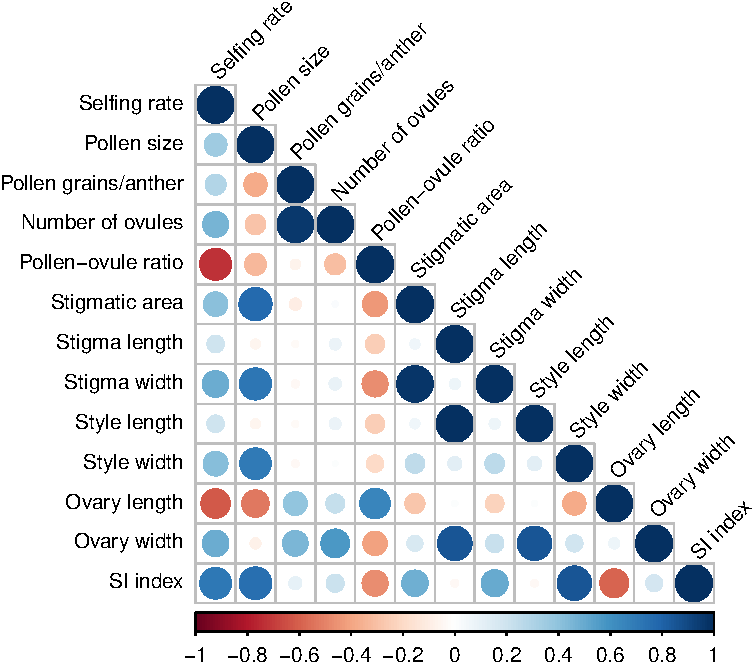
\includegraphics{Supp_Material_files/figure-latex/unnamed-chunk-14-1.pdf}
\caption{\textbf{Fig. S6} Graphical representation of the correlation
matrix of the different reproductive traits considered in the
experiment. Positive correlations are displayed in blue and negative in
red. The intensity, size and colour of the circles are proportional to
the correlation coefficient from Pearson's r.}
\end{figure}

\clearpage

\begin{figure}
\centering
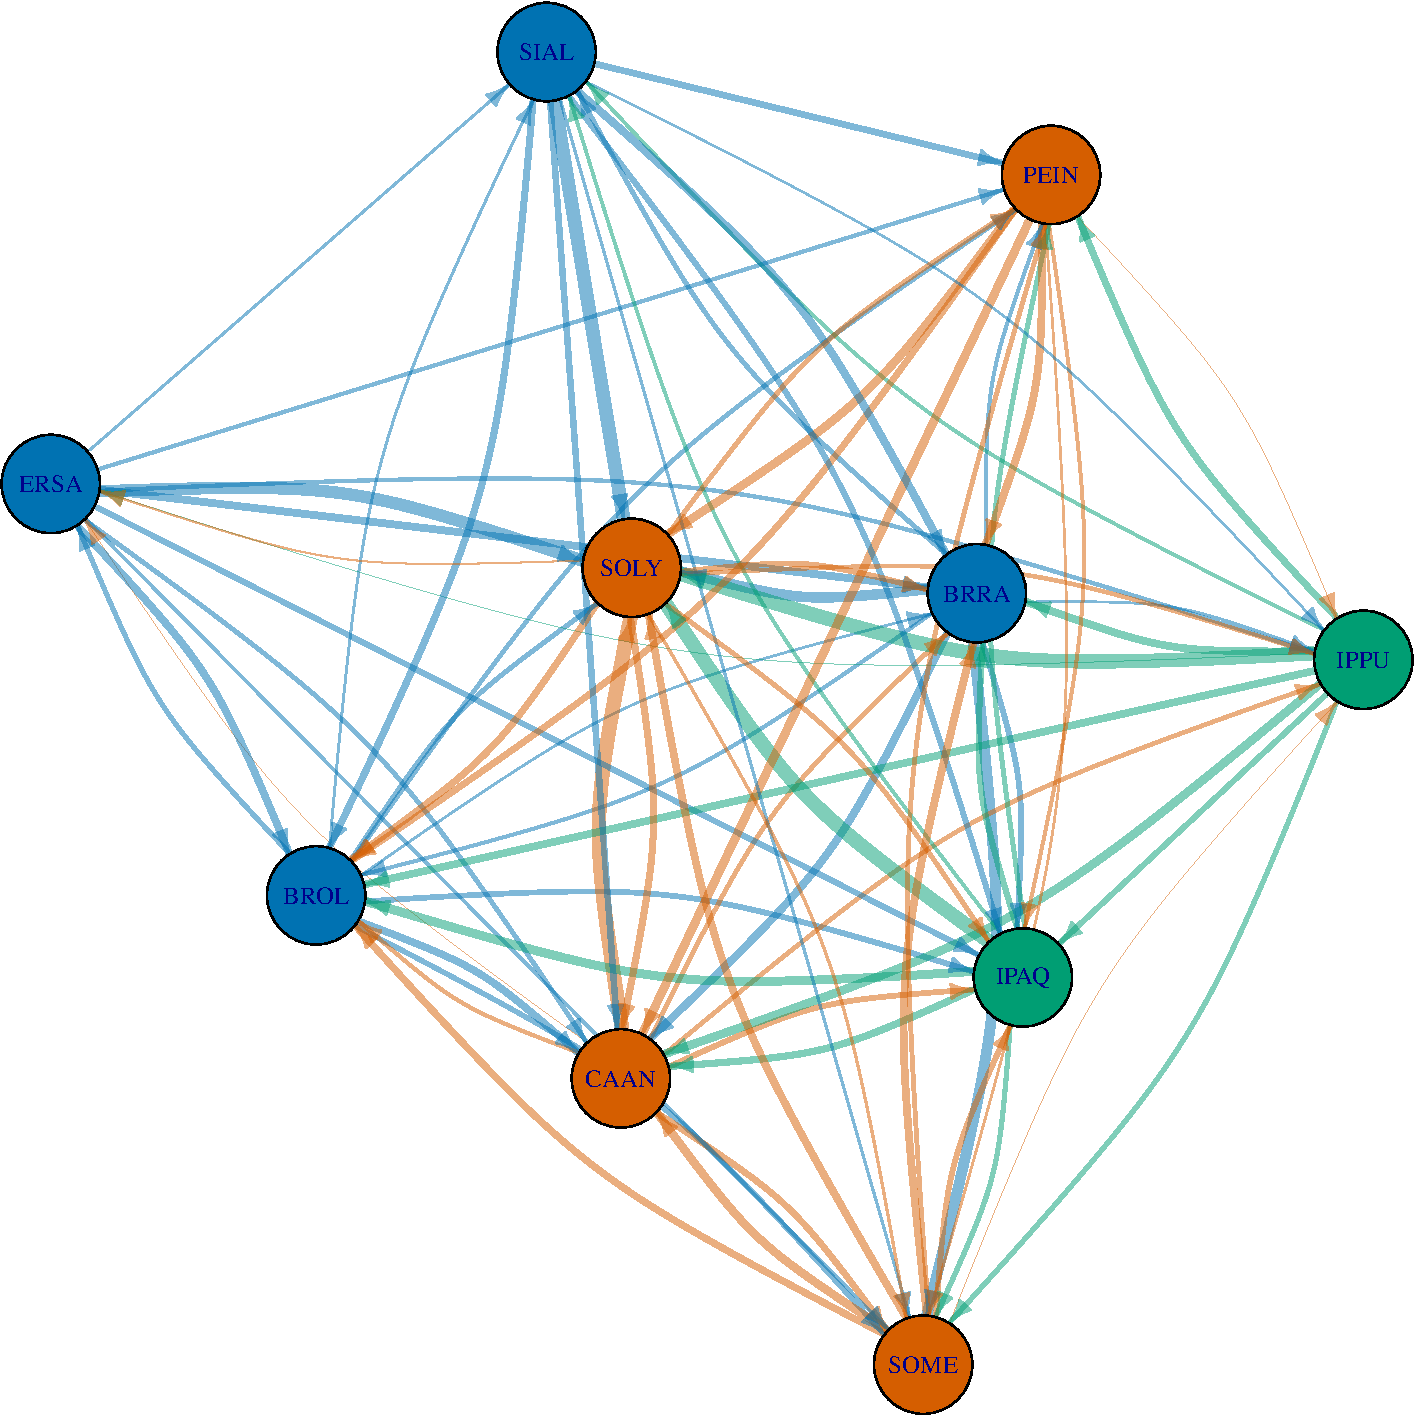
\includegraphics{Supp_Material_files/figure-latex/unnamed-chunk-15-1.pdf}
\caption{\textbf{Fig. S7} Violin plot of the proportion of seeds
coverted to ovule (\%) for all species with four different
hand-pollination treatments: apomixis (orange), hand cross pollination
(green), hand self pollination (blue) and spontaneous selfing (yellow).
The coloured dots, represent the different values of seed set for each
treatment.}
\end{figure}

\newpage

\begin{figure}
\centering
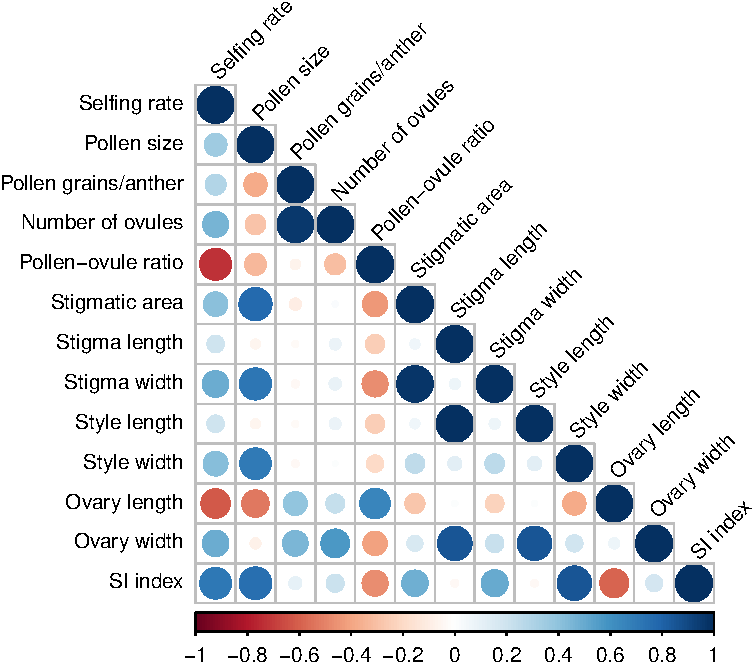
\includegraphics{Supp_Material_files/figure-latex/unnamed-chunk-16-1.pdf}
\caption{\textbf{Fig. S8} Grouped effect sizes (95\% confidence
intervals) of the different families on each focal species. For each
species, the grouped effect by family is compared with the control
treatment of hand cross pollination with conspecific pollen. The control
treatment is represented in yellow and vertically intersected with a
dashed line through the mean effect size in order to help the visual
interpretation of the effect sizes. Any value to the left of the
vertical dashed line represents a negative impact of foreign pollen. The
different effect sizes and confidence intervals are coloured by family:
Solanaceae (orange), Brassicaceae (blue) and Convolvulaceae (green).}
\end{figure}

\end{document}
